\section{Test Concept}
	Tests for all two main packages \textit{model} and \textit{view} have been created and executed, the created test cases can be found in the directory \textit{src/test/java/com.pathfinder.racetrack}. \\
	In the \textit{view} package, the different JavaFX GUI controllers (holding event handlers and more) are tested (e.g. \textit{OptionsMenuTest} or \textit{TracksMenuTest}) amongst all the helper classes for the view (e.g. \textit{ExceptionDialogTest} or \textit{JukeboxTest}). In the \textit{model} package, all the different used models are tested (e.g. \textit{GameEngineTest}, \textit{CarTest}, or \textit{VelocityTest}).\\~\\
	A total of \textbf{75} unique test cases are tested and verified with a total test coverage of \textcolor{ForestGreen}{\textbf{90\%}} on Class level, \textcolor{ForestGreen}{\textbf{87\%}} on Method level and \textcolor{ForestGreen}{\textbf{83\%}} on Line level, with all scopes exceeding the \textbf{80\%} test coverage threshold:
	\begin{figure}[H]
		\centering
		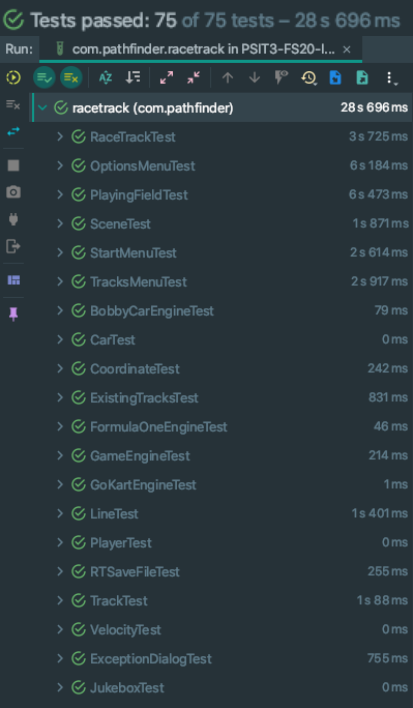
\includegraphics[width=8cm,keepaspectratio,center]{img/Implementation_Test-Concept_Test-Overview.png}
		\caption{Overview of test cases in RaceTrack}
	\end{figure}
	\begin{figure}[H]
		\centering
		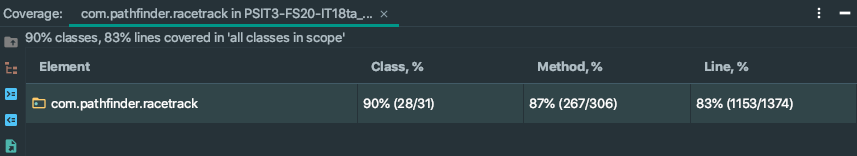
\includegraphics[width=12cm,keepaspectratio,center]{img/Implementation_Test-Concept_Coverage.png}
		\caption{Test Coverage in RaceTrack}
	\end{figure}
